\documentclass{article}

% if you need to pass options to natbib, use, e.g.:
%     \PassOptionsToPackage{numbers, compress}{natbib}
% before loading neurips_2021

% ready for submission
\usepackage[nonatbib]{neurips_2021}

% to compile a preprint version, e.g., for submission to arXiv, add add the
% [preprint] option:
%     \usepackage[preprint]{neurips_2021}

% to compile a camera-ready version, add the [final] option, e.g.:
%     \usepackage[final]{neurips_2021}

% to avoid loading the natbib package, add option nonatbib:
%    \usepackage[nonatbib]{neurips_2021}

\usepackage[utf8]{inputenc} % allow utf-8 input
\usepackage[T1]{fontenc}    % use 8-bit T1 fonts
\usepackage{hyperref}       % hyperlinks
\usepackage{url}            % simple URL typesetting
\usepackage{booktabs}       % professional-quality tables
\usepackage{amsfonts}       % blackboard math symbols
\usepackage{nicefrac}       % compact symbols for 1/2, etc.
\usepackage{microtype}      % m	Submitted ticrotypography
\usepackage{xcolor}         % colors
\usepackage{graphicx}
\usepackage{amsmath}
\usepackage{amssymb}

\DeclareRobustCommand{\bbone}{\text{\usefont{U}{bbold}{m}{n}1}}

\DeclareMathOperator{\EX}{\mathbb{E}}% expected value


\title{Benchmarking and reliability in RL}

% The \author macro works with any number of authors. There are two commands
% used to separate the names and addresses of multiple authors: \And and \AND.
%
% Using \And between authors leaves it to LaTeX to determine where to break the
% lines. Using \AND forces a line break at that point. So, if LaTeX puts 3 of 4
% authors names on the first line, and the last on the second line, try using
% \AND instead of \And before the third author name.

\author{Gurjeet Singh\\
  University of Padua\\
  \texttt{gurjeet.singh@studenti.unipd.it}
}

\begin{document}

\maketitle

\begin{abstract}
	We summarize in this paper pitfalls and issues of reinforcement learning models. We then report a recent paper in order effectively quantify agent's learning and allow to compare with different approaches.
	
\end{abstract}

\section{Introduction}
In the recent years there has been a great growth in the area of Deep Reinforcement Learning (DRL), novel approaches and techniques are constantly being invented and applied in many different domains.\\
But to progress in this field advanced studies have to be carried out on evaluation methods, in order to effectively compare model performances with pre-existing approaches. In such a manner we will able to detect and improve their weaknesses, and enhance results for further works.

Beside new reinforcement learning models there have been also an increasing growth for developing benchmarks and environments, even for the same agent's tasks there have been developed multiple environments.
Thanks to diverse benchmarking tests we are to able detect different aspects of the agent and to give a global picture of the learning by comparing them on different environments and across algorithms.

Despite the already existing benchmarks, it is still very hard to reproduce the results of Deep RL algorithms. At first we have to recall that reinforcement learning models have to deal most commonly with complex environments, which present strong stochasticity that could result into high variance and instability in the learning. However, still most of the issues and main causes of an algorithm to fail are because of the variance present in the learning algorithm, or either because of the variance incorporated in the dynamics of the environment.\\
In addition, as reported by Henderson et.al in their paper~\cite{DRL01}, the importance of reporting hyperparameters is essential to make the results of the experiments more reproducible, as highlighted by them just few changes on the configuration of neural network methods can lead in completely different results. In their studies, they have shown that many details of hyperparameters are not consistent and no ranges are provided, in addition, a lot experimental details are not reported leading to un-reproducible experiments. Thus being consistent and reporting the hyperparameters are extremely important to make the experiment reproducible.

In spite of the fact that more benchmarks are now released, there has not been defined a guideline or standardized method for fair comparisons among algorithms, and if tests are carried out poorly they can lead to misleading results. In addition, benchmarks are also used improperly and in a naive way for comparing different algorithms, indeed they should be exploited better, as we will see in this report.
For this reason, defining the appropriate metrics and statistical tests are essentially required to diagnose and compare different models approaches.\\
Indeed, we will discuss through this paper some recent measures and statistical, proposed by Google Research and Berkeley EECS~\cite{GoogleMeasure}, which are based on robust statistics and tests to assess the reliability and reproducibility of reinforcement learning model that deal with high instability in their results. Finally based on these measures they proposed a fair comparing method to evaluate different models that we will briefly discuss.


\section{Method}
In this section, we state past and recent measures and test methodologies proposed in the scientific literature to assess evaluation methods of reinforcement learning models. For each approach we describe the proposed method but also their usage, aims, explanatory power, and highlight issues related to the measures and their applications.
\paragraph{Common metrics}
As mentioned in the Introduction in Reinforcement learning models reproducing an experiment is a challenging problem and it requires specific metrics, in order to carry our simulations and replicate results in some experiments.
A common evaluation metric in RL algorithms is the average cumulative reward over some episodes $T$, i.e the average returns, and it is defined as:	
\begin{equation}
G(A) = \EX_{s_{t+1} \sim f} \left[\sum_{t=0}^{T} r(s_t, a_t)\right].	
\end{equation}

Other metrics like maximum reward achieve over a fixed number of time steps have been also used, but  due to the unstable nature of many algorithms, reporting maximums return is inadequate. Even reporting only the average returns results to be misleading, in fact they have to be combined at least with the confidence intervals (CI).
\paragraph{Confidence intervals}
By adding the CI we are able to track the variance present in the average return in our samples during training and test phases. This measure can be helpful as a first evaluation for simple comparison among different algorithms.\\ But most importantly, thanks to it, we are able to tune important hyperparameters of the algorithm. In addition, it also allows to detect some pitfalls in the learning of the agent. In fact, it has been shown from paper~\cite{DRL01}, that variance between runs of a model can be enough to create statistically different distribution just by varying the random seed across trials or by applying different simulation on the test set, which can be easily detect by plotting the average returns with the relative confidence interval from different runs.
This issue can even happen by averaging several learning results together across different random seed.\\
The major cause of this problem can be associated with the variance present in the environment or in the learning process, but it can be mostly caused also by the chosen sample size that is not enough to have a consistent learning behaviour across different runs.
\paragraph{Power Analysis}
To overcome this problem we can apply power analysis and statistical test in order to understand the required sample size or episodes such that the performances have same distribution across different runs.\\
An example of sample size analysis is bootstrap power analysis~\cite{pwranaly2} as suggested by Henderson et.al \cite{DRL01} in their work, which is used by running many bootstrap simulation and determine the percentage of the simulations result in statistically significant values, where in case of low percentage of significant values a large sample size is required in each run. But a full detail on sample size study for RL problems can be found in the chapter 3 and 4 of Colas et.al paper~\cite{PowerAnalysis}, where they used Welch's t-test and power analysis methods to understand the sample size required by the model.
\paragraph{Multiple Environments}
Another type of inconsistency in performances of RL models regards multi-environments tests which have been highlighted first from Henderson's work~\cite{DRL01}, and further analysis has also been done in Helfenstein's paper~\cite{BenchmarkingDRL}.  In both works, it has been shown that evaluation of models across different environment are barely addressed and tested. 
They have found that algorithms performances can differ significantly depending on the chosen environment, leading to misleading results when comparing different algorithms. Thus, it should be more considered not just test the model on a single environments but also compare the learning of the agent on multiple environments in order to understand their variance and reliability.\\
In their papers some of the causes of this issue have also been detected, they addressed two major factors, the presence of biases in the learning of the agent or because of preprocessing techniques applied on the environment. Indeed, in their experiments they found that biases in the agent can be introduced with reward scaling normalization layers which can have a large effect in gradient based methods. Large and sparse output scale can result in problem regarding saturation and inefficiency in the learning, thus compressing the space of estimated expected returns in action value function based method using reward scaling can be very fruitful to agent. But results are inconsistent across environments causing failure to learn on unstable environment where Deep Q-Value function approximator are used or where untuned reward scales are defined. To overcome this issues a better approach would be to adaptively rescale reward targets with normalized stochastic gradient a made by Van Hasselt et.al in their work ~\cite{VaHasselt}.
\paragraph{MBRL}
All the previous issues and methods are applied to any Reinforcement Learning algorithm, but when considering Model-based Reinforcement Learning (MBRL) more tests are required to carry out. These type of algorithm have the potential to be significantly more sample efficient by modelling the transition dynamic. But research in this particular field has not been very standardized. Indeed, it is common that experiments are carried out with self-designed environment, which are sometimes closed-sourced, leading to un-reproducible algorithms.\\
For this reason in Wang et.al work ~\cite{MBRLBenchmarking} have addressed this issue by proposing new benchmark environments designed for MBRL. They adapted many common environments of model-free RL for MBRL, because
contrary to free model approaches, MBRL requires access to an analytics differentiable reward function, such that the gradient can be compute. For this reason in their work they adapted the environment by adapting or approximating the reward functions in order to make them differentiable.\\
In their work, they also 


\paragraph{Robust statistics and reliability}
As we have seen through different proposed approaches and issues, reliability is a major problem in RL algorithms. Recently, thanks to  Berkeley EECS and Google Research collaboration, some efforts have been made into defining adequate metric to quantify different aspect of reliability. In their work~\cite{GoogleMeasure}, they designed statistical test for enabling rigorous comparisons of algorithms by using robust statistics. These metrics measure the reliability by looking at different aspects: reproducibility, stability, variability/dispersion, and risk.\\
All these properties can be detected by measuring dispersion, and risk of the average rewards. The former one, measure the width of the distribution and it is inferred using the \textbf{Inter-quartile range (IQR)}, i.e the difference between the 75th and 25th percentile, $ IQR(X) = Q_3(X) - Q_1(X)$, this metric does not require assuming normality of the distribution and it is suitable for asymmetric distribution.
Instead, Risk can be derived by quantifying the heaviness and extend of the lower tail of the distribution, which give us the worst-case scenarios of the performances. To measure it \textbf{Conditional Value at Risk (CVaR)} can be used and it is defined as:
\begin{equation}
CVaR_\alpha(X) = \EX \left[ X \vert X \leq Var_\alpha(X) \right]  \quad \alpha \in (0,1)
\end{equation}
Where $VaR_\alpha$ is the value at Risk, i.e the $\alpha$-quantile of distribution $X$ and it is defined as:
\begin{equation}
VaR_\alpha(X) = -inf \{ x \in \mathbb{R}: F_X(x) \ge \alpha \}
\end{equation}

By applying the previous metrics on different phases we can extract several information, as summarized by the following Table \ref{fig:table}.
\begin{figure}[!htp]
	\centering
	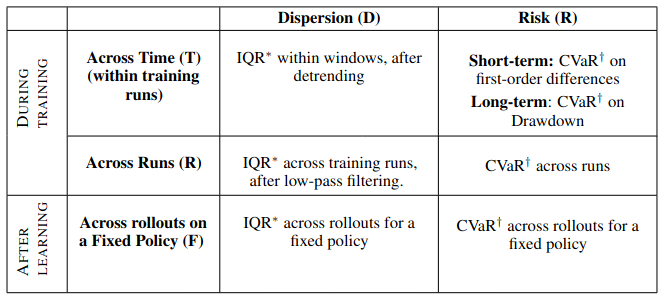
\includegraphics[scale=0.3]{./images/table.png}
	\caption{Summary of proposed reliability metrics~\cite{GoogleMeasure}}
	\label{fig:table}
	\footnotesize{}
\end{figure}
At first we distinguish two phases, during training and after learning.
Within training runs (across time, within each run) we check the stability across time by looking for monotonic improvement in the measures.
The IQR across time is applied using a sliding window on detrended training, i.e $y_{t'} = y_{t} - y_{t-1}$, to not capture long term trend and isolate higher frequency variability.
Instead, short term risk measures the most extreme short-term drop over time, by applying the $CVaR_\alpha$ on a distribution obtained by the differences of one point of evaluation to the next one normalized by the distance between time-point $CVaR_\alpha \left(\frac{X_t - X_{t+n}}{n}\right)$, to make it invariance to evaluation frequency.\\
On the other hand, long term risk is obtained by looking at the draw-down at time T, which describes the drop in performance relative to the highest peak so far this way we capture drop over longer timescale but also unusual short term drops.\\
By contrast, when analyzing the model across runs, we should have reproducible performances and consistency. Here the variability describes the algorithm’s sensitivity to random seed which includes initialization of weights, and sensitivity to multiple environments. The $CVaR$ during this phase gives the expected worst performances across all the runs.\\
Once fixing the policy, i.e after learning, the two measures allow to measure the reproducibility of the algorithm by comparing it with the results across runs during the training phase.

Thanks to these reliability metrics we are able to quantify different aspects of an algorithm and they can help to pinpoint their specific strengths and weaknesses. But when we need to compare different models and consider multiple environments, the metrics can not be compared directly.
The results can have different ranges and distribution of reward across multiple environments, thus a suggested approach is to compute the median range of performance. In addition, for a fair comparison of multiple algorithms, ranking method of the agent with related statistical test has been proposed by Chan et.al~\cite{GoogleMeasure}. In their paper, they designed a pair permutation test applied after ranking the algorithm for each agent's task on per run-metrics or across run. The permutation test is based on bootstrap sampling on the ranking, and by applying mean ranking on each resample, we can obtain a distribution over the ranking, by making difference between the metric ranking of the two algorithms, assuming under the null hypothesis that runs/episodes are exchangeable. Thus from the retrieved distribution we can apply the statistical test and p-value thresholding for rejecting or not the observed value. The statistical test can be summarized as follow:
\begin{equation}
\begin{split}
	&S_{MetricRanking}(A, B) = MetricRanking (A) - MetricRanking (B) \\
	&H_0 : S_{MetricRanking}(A, B) =  0 \\
	&H_1 : S_{MetricRanking}(A, B) \neq  0 \\
	&(A', B')\in P (A \cup B) \quad S_{MetricRanking}(A', B')
\end{split}
\end{equation}
Where, $MetricRanking$ is the mean of reliability metric ranking across tasks. Instead, $A$ and $B$ are sets of performance measurements (e.g average return) for the first and second algorithms. Lastly, bootstrap sampling is applied on the permutations of $ S_{MetricRanking}(A', B')$ statistics to obtain a distribution and finally apply the statistical test on the observed value.\\
The authors of this method have been able to found, in their experimental analysis, that reliability is a separate dimension, which needs to be inspected separately from mean or median performance, i.e two algorithms may have similar median performance, but may nonetheless significantly differ in reliability. Additionally, they have proved that reliability along one axis (e.g across time) does not necessarily correlate with reliability on the other two axes (e.g across runs or roll-outs).\\
All these proposed metrics and statistical test have been made available as an open-source library\footnote{https://github.com/google-research/rl-reliability-metrics} with a few required hyperparameters that have to be reported in the experiments to ensure reproducibility.
\label{gen_inst}
\section{Experiments}
From the methods described in the previous section, different experiments have been carried out by each author in order to prove their results and highlight the issues present in some algorithms. For this reason, we report in this paper some meaningful results to give some insights and usage of the metrics and methods discussed previously.

\paragraph{Sample size}
As mentioned in the first part of the Method section, the confidence interval is the simplest measure that has been considered when using RL models. Although its simplicity, it can be used to tune major hyperparameters of an algorithm and can highlight also the learning progress of the agent, but even some of its pitfalls. An example of its usage can be seen in the following Figure ~\ref{fig:sample_size} from Henderson et.al work. In this plot, we can see an example of reporting the CI, but also the instability of the TRPO \cite{TRPO} algorithm detected by using the same hyperparameter configuration proposed by the original paper on the HalfCheetah-v1 agent of OpenAI Gym environment. This result shows the inconsistency of the algorithms even by averaging the models across two different sets of runs. As we previously see, this issue can be overcome by applying power analysis tests to estimate the required sample size for a consistent learning behaviour and avoid statistically different distributions of the average return for the same algorithm across runs.
\begin{figure}[!]
	\centering
	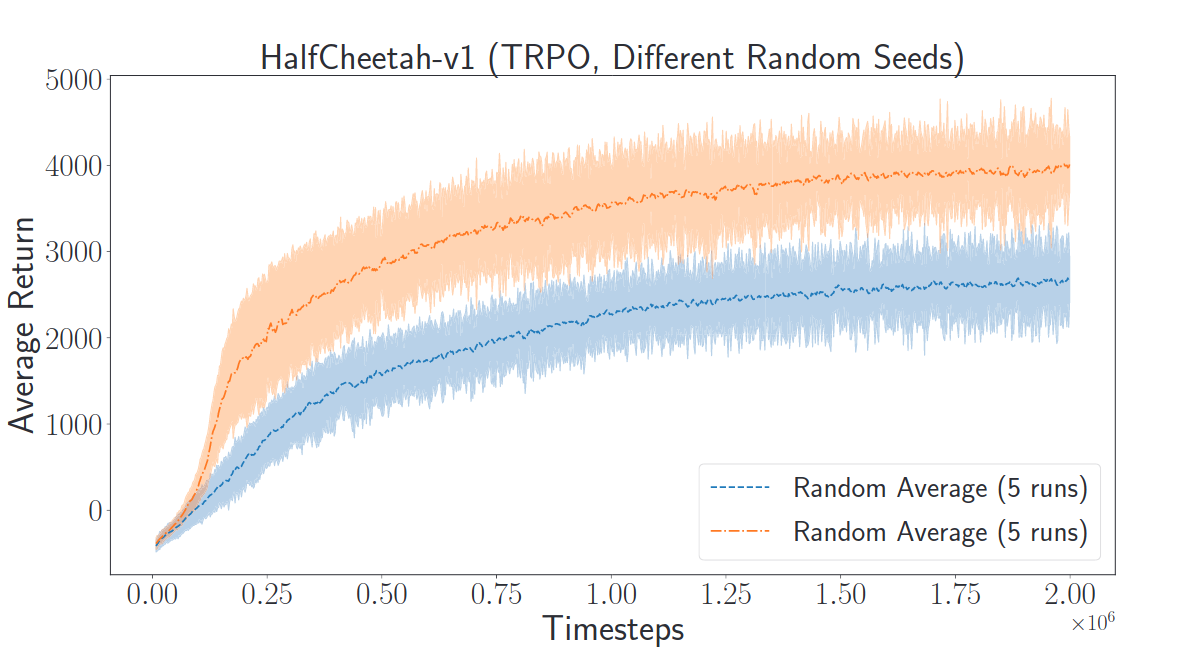
\includegraphics[scale=0.15]{./images/sample_size_dist.png}
	\caption{TRPO on HalfCheetah-v1~\cite{DRL01}}
	\label{fig:sample_size}
\end{figure}

\paragraph{Environment}
Another important type of assessment which is less likely done but should be considered more is to evaluate the consistency of the model on different environments. These type of tests have been studied by Helfenstein in his experimental works.~\cite{BenchmarkingDRL}. An example of his results can be seen in the following plot \ref{fig:env}. In this experiment, the performances of some free RL models for the Hopper agent on three different environment implementations: OpenAI Gym, PyBullet, and DeepMind. This plot shows the inconsistency of  models across multiple environments, indeed for the same task, the algorithm performances can differ significantly depending on the chosen environment, as shown from the rewards and the instability of the algorithms in the plot.
The SAC model in all the scenarios has a very fast initial learning behaviour, but in the first environment its performances drop by ending as the third worst final undiscounted return, since it maximizes the immediate short-term reward. Instead, other algorithms take more in consideration the bonus given in the reward for staying alive. In PyBullet instead, SAC stays constantly higher than the others, and in DeepMind it is the only algorithm able to show some learning behaviour. Indeed, DeepMind is the hardest environment comparing all the others, because it does not give bonus on reward by staying alive.

\begin{figure*}[!htp]
	\centering
	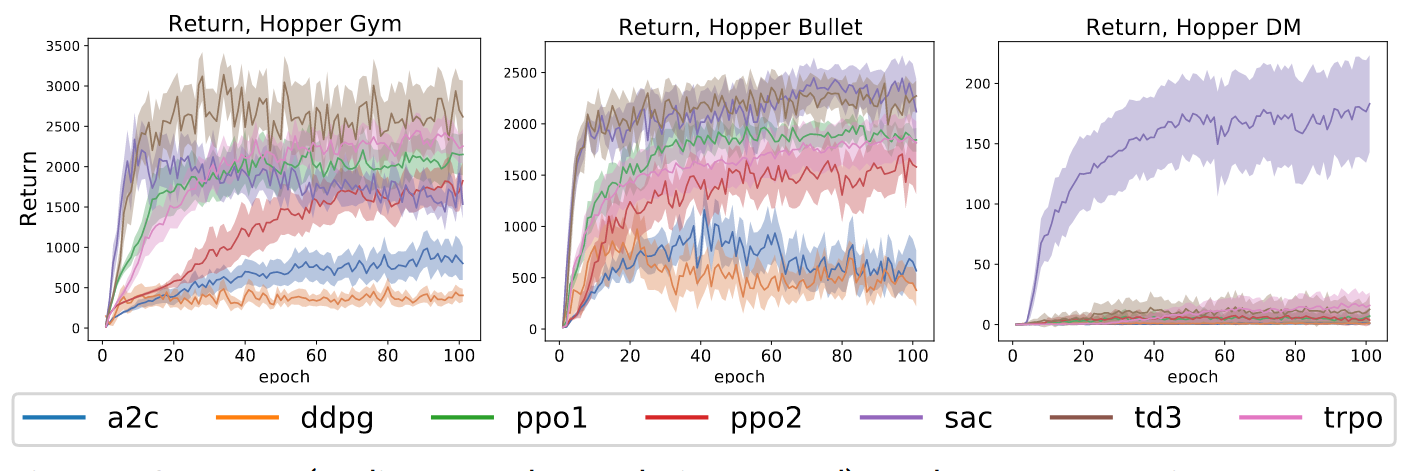
\includegraphics[scale=0.3]{./images/Environements_plot.png}
	\caption{Environment inconsistency \cite{BenchmarkingDRL}}
	\label{fig:env}
	\footnotesize{}
\end{figure*}
\paragraph{Reliability}
In order to prove the separate dimension of reliability from mean and median performances we report an experiment made by Chan et.al using their novel approach based on robust statics. The experiment involved the comparison of four different variant of Deep Q-Leaning algorithms (DQN, IQN, C51, Rainbow ~\cite{DQN, IQN, C51,Rainbow}) on 60 Atari games. As shown in summary plot \ref{fig:realibility} even though Rainbow performs significantly better than IQN in Median Performance, IQN performs numerically or significantly better than Rainbow on many of the reliability metrics. Thus the novel proposed measures demonstrate the reliability as a different dimension. Further analysis and  statistical permutation test on different experiments can be found in the supplemental material of their work.

\begin{figure}[!htp]
	\centering
	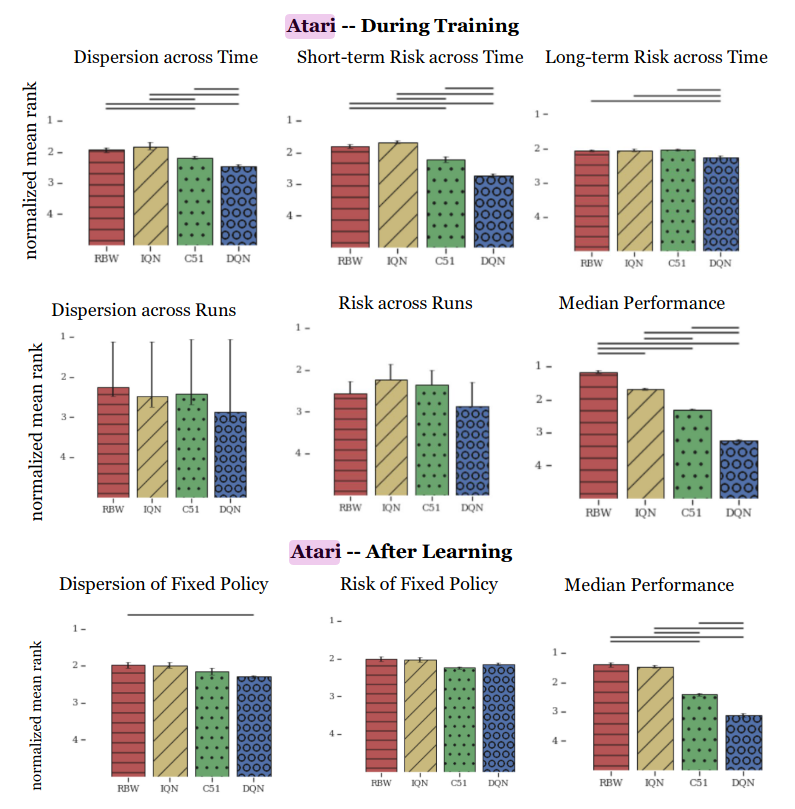
\includegraphics[scale=0.3]{./images/atari_ranking.png}
	\caption{Ranking of reliability metrics on 60 Atari games~\cite{GoogleMeasure}}
	\label{fig:realibility}
	\footnotesize{}
\end{figure}


\section{Conclusion}
In this paper we have seen different issues and aspects of reproducibility and evaluation criteria on RL models. In particular, we have seen novel measures and tests based on robust statistics  for evaluating reliability of a model, which is obscured to mean and median metrics. Thanks to all these methods, we are able to give more explanatory power of RL models results, in addition, they allow to understand strengths and weaknesses of the model, in order to improve existing algorithm, but also for suggesting future works for building robust, and reliable models.\\
We hope that more research and focus will be done on robust metrics to implement reliable and reproducible models.

practical recommendations for the evaluating models.
\clearpage


\section{Appendix}

Optionally include extra information (complete proofs, additional experiments and plots) in the appendix.
This section will often be part of the supplemental material.

{\small
	\bibliographystyle{ieee_fullname}
	\bibliography{egbib}
}

\appendix

\end{document}
